\documentclass[11pt]{article}

    \usepackage[breakable]{tcolorbox}
    \usepackage{parskip} % Stop auto-indenting (to mimic markdown behaviour)
    
    \usepackage{iftex}
    \ifPDFTeX
    	\usepackage[T1]{fontenc}
    	\usepackage{mathpazo}
    \else
    	\usepackage{fontspec}
    \fi

    % Basic figure setup, for now with no caption control since it's done
    % automatically by Pandoc (which extracts ![](path) syntax from Markdown).
    \usepackage{graphicx}
    % Maintain compatibility with old templates. Remove in nbconvert 6.0
    \let\Oldincludegraphics\includegraphics
    % Ensure that by default, figures have no caption (until we provide a
    % proper Figure object with a Caption API and a way to capture that
    % in the conversion process - todo).
    \usepackage{caption}
    \DeclareCaptionFormat{nocaption}{}
    \captionsetup{format=nocaption,aboveskip=0pt,belowskip=0pt}

    \usepackage{float}
    \floatplacement{figure}{H} % forces figures to be placed at the correct location
    \usepackage{xcolor} % Allow colors to be defined
    \usepackage{enumerate} % Needed for markdown enumerations to work
    \usepackage{geometry} % Used to adjust the document margins
    \usepackage{amsmath} % Equations
    \usepackage{amssymb} % Equations
    \usepackage{textcomp} % defines textquotesingle
    % Hack from http://tex.stackexchange.com/a/47451/13684:
    \AtBeginDocument{%
        \def\PYZsq{\textquotesingle}% Upright quotes in Pygmentized code
    }
    \usepackage{upquote} % Upright quotes for verbatim code
    \usepackage{eurosym} % defines \euro
    \usepackage[mathletters]{ucs} % Extended unicode (utf-8) support
    \usepackage{fancyvrb} % verbatim replacement that allows latex
    \usepackage{grffile} % extends the file name processing of package graphics 
                         % to support a larger range
    \makeatletter % fix for old versions of grffile with XeLaTeX
    \@ifpackagelater{grffile}{2019/11/01}
    {
      % Do nothing on new versions
    }
    {
      \def\Gread@@xetex#1{%
        \IfFileExists{"\Gin@base".bb}%
        {\Gread@eps{\Gin@base.bb}}%
        {\Gread@@xetex@aux#1}%
      }
    }
    \makeatother
    \usepackage[Export]{adjustbox} % Used to constrain images to a maximum size
    \adjustboxset{max size={0.9\linewidth}{0.9\paperheight}}

    % The hyperref package gives us a pdf with properly built
    % internal navigation ('pdf bookmarks' for the table of contents,
    % internal cross-reference links, web links for URLs, etc.)
    \usepackage{hyperref}
    % The default LaTeX title has an obnoxious amount of whitespace. By default,
    % titling removes some of it. It also provides customization options.
    \usepackage{titling}
    \usepackage{longtable} % longtable support required by pandoc >1.10
    \usepackage{booktabs}  % table support for pandoc > 1.12.2
    \usepackage[inline]{enumitem} % IRkernel/repr support (it uses the enumerate* environment)
    \usepackage[normalem]{ulem} % ulem is needed to support strikethroughs (\sout)
                                % normalem makes italics be italics, not underlines
    \usepackage{mathrsfs}
    

    
    % Colors for the hyperref package
    \definecolor{urlcolor}{rgb}{0,.145,.698}
    \definecolor{linkcolor}{rgb}{.71,0.21,0.01}
    \definecolor{citecolor}{rgb}{.12,.54,.11}

    % ANSI colors
    \definecolor{ansi-black}{HTML}{3E424D}
    \definecolor{ansi-black-intense}{HTML}{282C36}
    \definecolor{ansi-red}{HTML}{E75C58}
    \definecolor{ansi-red-intense}{HTML}{B22B31}
    \definecolor{ansi-green}{HTML}{00A250}
    \definecolor{ansi-green-intense}{HTML}{007427}
    \definecolor{ansi-yellow}{HTML}{DDB62B}
    \definecolor{ansi-yellow-intense}{HTML}{B27D12}
    \definecolor{ansi-blue}{HTML}{208FFB}
    \definecolor{ansi-blue-intense}{HTML}{0065CA}
    \definecolor{ansi-magenta}{HTML}{D160C4}
    \definecolor{ansi-magenta-intense}{HTML}{A03196}
    \definecolor{ansi-cyan}{HTML}{60C6C8}
    \definecolor{ansi-cyan-intense}{HTML}{258F8F}
    \definecolor{ansi-white}{HTML}{C5C1B4}
    \definecolor{ansi-white-intense}{HTML}{A1A6B2}
    \definecolor{ansi-default-inverse-fg}{HTML}{FFFFFF}
    \definecolor{ansi-default-inverse-bg}{HTML}{000000}

    % common color for the border for error outputs.
    \definecolor{outerrorbackground}{HTML}{FFDFDF}

    % commands and environments needed by pandoc snippets
    % extracted from the output of `pandoc -s`
    \providecommand{\tightlist}{%
      \setlength{\itemsep}{0pt}\setlength{\parskip}{0pt}}
    \DefineVerbatimEnvironment{Highlighting}{Verbatim}{commandchars=\\\{\}}
    % Add ',fontsize=\small' for more characters per line
    \newenvironment{Shaded}{}{}
    \newcommand{\KeywordTok}[1]{\textcolor[rgb]{0.00,0.44,0.13}{\textbf{{#1}}}}
    \newcommand{\DataTypeTok}[1]{\textcolor[rgb]{0.56,0.13,0.00}{{#1}}}
    \newcommand{\DecValTok}[1]{\textcolor[rgb]{0.25,0.63,0.44}{{#1}}}
    \newcommand{\BaseNTok}[1]{\textcolor[rgb]{0.25,0.63,0.44}{{#1}}}
    \newcommand{\FloatTok}[1]{\textcolor[rgb]{0.25,0.63,0.44}{{#1}}}
    \newcommand{\CharTok}[1]{\textcolor[rgb]{0.25,0.44,0.63}{{#1}}}
    \newcommand{\StringTok}[1]{\textcolor[rgb]{0.25,0.44,0.63}{{#1}}}
    \newcommand{\CommentTok}[1]{\textcolor[rgb]{0.38,0.63,0.69}{\textit{{#1}}}}
    \newcommand{\OtherTok}[1]{\textcolor[rgb]{0.00,0.44,0.13}{{#1}}}
    \newcommand{\AlertTok}[1]{\textcolor[rgb]{1.00,0.00,0.00}{\textbf{{#1}}}}
    \newcommand{\FunctionTok}[1]{\textcolor[rgb]{0.02,0.16,0.49}{{#1}}}
    \newcommand{\RegionMarkerTok}[1]{{#1}}
    \newcommand{\ErrorTok}[1]{\textcolor[rgb]{1.00,0.00,0.00}{\textbf{{#1}}}}
    \newcommand{\NormalTok}[1]{{#1}}
    
    % Additional commands for more recent versions of Pandoc
    \newcommand{\ConstantTok}[1]{\textcolor[rgb]{0.53,0.00,0.00}{{#1}}}
    \newcommand{\SpecialCharTok}[1]{\textcolor[rgb]{0.25,0.44,0.63}{{#1}}}
    \newcommand{\VerbatimStringTok}[1]{\textcolor[rgb]{0.25,0.44,0.63}{{#1}}}
    \newcommand{\SpecialStringTok}[1]{\textcolor[rgb]{0.73,0.40,0.53}{{#1}}}
    \newcommand{\ImportTok}[1]{{#1}}
    \newcommand{\DocumentationTok}[1]{\textcolor[rgb]{0.73,0.13,0.13}{\textit{{#1}}}}
    \newcommand{\AnnotationTok}[1]{\textcolor[rgb]{0.38,0.63,0.69}{\textbf{\textit{{#1}}}}}
    \newcommand{\CommentVarTok}[1]{\textcolor[rgb]{0.38,0.63,0.69}{\textbf{\textit{{#1}}}}}
    \newcommand{\VariableTok}[1]{\textcolor[rgb]{0.10,0.09,0.49}{{#1}}}
    \newcommand{\ControlFlowTok}[1]{\textcolor[rgb]{0.00,0.44,0.13}{\textbf{{#1}}}}
    \newcommand{\OperatorTok}[1]{\textcolor[rgb]{0.40,0.40,0.40}{{#1}}}
    \newcommand{\BuiltInTok}[1]{{#1}}
    \newcommand{\ExtensionTok}[1]{{#1}}
    \newcommand{\PreprocessorTok}[1]{\textcolor[rgb]{0.74,0.48,0.00}{{#1}}}
    \newcommand{\AttributeTok}[1]{\textcolor[rgb]{0.49,0.56,0.16}{{#1}}}
    \newcommand{\InformationTok}[1]{\textcolor[rgb]{0.38,0.63,0.69}{\textbf{\textit{{#1}}}}}
    \newcommand{\WarningTok}[1]{\textcolor[rgb]{0.38,0.63,0.69}{\textbf{\textit{{#1}}}}}
    
    
    % Define a nice break command that doesn't care if a line doesn't already
    % exist.
    \def\br{\hspace*{\fill} \\* }
    % Math Jax compatibility definitions
    \def\gt{>}
    \def\lt{<}
    \let\Oldtex\TeX
    \let\Oldlatex\LaTeX
    \renewcommand{\TeX}{\textrm{\Oldtex}}
    \renewcommand{\LaTeX}{\textrm{\Oldlatex}}
    % Document parameters
    % Document title
    \title{chapter-3-1}
    
    
    
    
    
% Pygments definitions
\makeatletter
\def\PY@reset{\let\PY@it=\relax \let\PY@bf=\relax%
    \let\PY@ul=\relax \let\PY@tc=\relax%
    \let\PY@bc=\relax \let\PY@ff=\relax}
\def\PY@tok#1{\csname PY@tok@#1\endcsname}
\def\PY@toks#1+{\ifx\relax#1\empty\else%
    \PY@tok{#1}\expandafter\PY@toks\fi}
\def\PY@do#1{\PY@bc{\PY@tc{\PY@ul{%
    \PY@it{\PY@bf{\PY@ff{#1}}}}}}}
\def\PY#1#2{\PY@reset\PY@toks#1+\relax+\PY@do{#2}}

\@namedef{PY@tok@w}{\def\PY@tc##1{\textcolor[rgb]{0.73,0.73,0.73}{##1}}}
\@namedef{PY@tok@c}{\let\PY@it=\textit\def\PY@tc##1{\textcolor[rgb]{0.25,0.50,0.50}{##1}}}
\@namedef{PY@tok@cp}{\def\PY@tc##1{\textcolor[rgb]{0.74,0.48,0.00}{##1}}}
\@namedef{PY@tok@k}{\let\PY@bf=\textbf\def\PY@tc##1{\textcolor[rgb]{0.00,0.50,0.00}{##1}}}
\@namedef{PY@tok@kp}{\def\PY@tc##1{\textcolor[rgb]{0.00,0.50,0.00}{##1}}}
\@namedef{PY@tok@kt}{\def\PY@tc##1{\textcolor[rgb]{0.69,0.00,0.25}{##1}}}
\@namedef{PY@tok@o}{\def\PY@tc##1{\textcolor[rgb]{0.40,0.40,0.40}{##1}}}
\@namedef{PY@tok@ow}{\let\PY@bf=\textbf\def\PY@tc##1{\textcolor[rgb]{0.67,0.13,1.00}{##1}}}
\@namedef{PY@tok@nb}{\def\PY@tc##1{\textcolor[rgb]{0.00,0.50,0.00}{##1}}}
\@namedef{PY@tok@nf}{\def\PY@tc##1{\textcolor[rgb]{0.00,0.00,1.00}{##1}}}
\@namedef{PY@tok@nc}{\let\PY@bf=\textbf\def\PY@tc##1{\textcolor[rgb]{0.00,0.00,1.00}{##1}}}
\@namedef{PY@tok@nn}{\let\PY@bf=\textbf\def\PY@tc##1{\textcolor[rgb]{0.00,0.00,1.00}{##1}}}
\@namedef{PY@tok@ne}{\let\PY@bf=\textbf\def\PY@tc##1{\textcolor[rgb]{0.82,0.25,0.23}{##1}}}
\@namedef{PY@tok@nv}{\def\PY@tc##1{\textcolor[rgb]{0.10,0.09,0.49}{##1}}}
\@namedef{PY@tok@no}{\def\PY@tc##1{\textcolor[rgb]{0.53,0.00,0.00}{##1}}}
\@namedef{PY@tok@nl}{\def\PY@tc##1{\textcolor[rgb]{0.63,0.63,0.00}{##1}}}
\@namedef{PY@tok@ni}{\let\PY@bf=\textbf\def\PY@tc##1{\textcolor[rgb]{0.60,0.60,0.60}{##1}}}
\@namedef{PY@tok@na}{\def\PY@tc##1{\textcolor[rgb]{0.49,0.56,0.16}{##1}}}
\@namedef{PY@tok@nt}{\let\PY@bf=\textbf\def\PY@tc##1{\textcolor[rgb]{0.00,0.50,0.00}{##1}}}
\@namedef{PY@tok@nd}{\def\PY@tc##1{\textcolor[rgb]{0.67,0.13,1.00}{##1}}}
\@namedef{PY@tok@s}{\def\PY@tc##1{\textcolor[rgb]{0.73,0.13,0.13}{##1}}}
\@namedef{PY@tok@sd}{\let\PY@it=\textit\def\PY@tc##1{\textcolor[rgb]{0.73,0.13,0.13}{##1}}}
\@namedef{PY@tok@si}{\let\PY@bf=\textbf\def\PY@tc##1{\textcolor[rgb]{0.73,0.40,0.53}{##1}}}
\@namedef{PY@tok@se}{\let\PY@bf=\textbf\def\PY@tc##1{\textcolor[rgb]{0.73,0.40,0.13}{##1}}}
\@namedef{PY@tok@sr}{\def\PY@tc##1{\textcolor[rgb]{0.73,0.40,0.53}{##1}}}
\@namedef{PY@tok@ss}{\def\PY@tc##1{\textcolor[rgb]{0.10,0.09,0.49}{##1}}}
\@namedef{PY@tok@sx}{\def\PY@tc##1{\textcolor[rgb]{0.00,0.50,0.00}{##1}}}
\@namedef{PY@tok@m}{\def\PY@tc##1{\textcolor[rgb]{0.40,0.40,0.40}{##1}}}
\@namedef{PY@tok@gh}{\let\PY@bf=\textbf\def\PY@tc##1{\textcolor[rgb]{0.00,0.00,0.50}{##1}}}
\@namedef{PY@tok@gu}{\let\PY@bf=\textbf\def\PY@tc##1{\textcolor[rgb]{0.50,0.00,0.50}{##1}}}
\@namedef{PY@tok@gd}{\def\PY@tc##1{\textcolor[rgb]{0.63,0.00,0.00}{##1}}}
\@namedef{PY@tok@gi}{\def\PY@tc##1{\textcolor[rgb]{0.00,0.63,0.00}{##1}}}
\@namedef{PY@tok@gr}{\def\PY@tc##1{\textcolor[rgb]{1.00,0.00,0.00}{##1}}}
\@namedef{PY@tok@ge}{\let\PY@it=\textit}
\@namedef{PY@tok@gs}{\let\PY@bf=\textbf}
\@namedef{PY@tok@gp}{\let\PY@bf=\textbf\def\PY@tc##1{\textcolor[rgb]{0.00,0.00,0.50}{##1}}}
\@namedef{PY@tok@go}{\def\PY@tc##1{\textcolor[rgb]{0.53,0.53,0.53}{##1}}}
\@namedef{PY@tok@gt}{\def\PY@tc##1{\textcolor[rgb]{0.00,0.27,0.87}{##1}}}
\@namedef{PY@tok@err}{\def\PY@bc##1{{\setlength{\fboxsep}{\string -\fboxrule}\fcolorbox[rgb]{1.00,0.00,0.00}{1,1,1}{\strut ##1}}}}
\@namedef{PY@tok@kc}{\let\PY@bf=\textbf\def\PY@tc##1{\textcolor[rgb]{0.00,0.50,0.00}{##1}}}
\@namedef{PY@tok@kd}{\let\PY@bf=\textbf\def\PY@tc##1{\textcolor[rgb]{0.00,0.50,0.00}{##1}}}
\@namedef{PY@tok@kn}{\let\PY@bf=\textbf\def\PY@tc##1{\textcolor[rgb]{0.00,0.50,0.00}{##1}}}
\@namedef{PY@tok@kr}{\let\PY@bf=\textbf\def\PY@tc##1{\textcolor[rgb]{0.00,0.50,0.00}{##1}}}
\@namedef{PY@tok@bp}{\def\PY@tc##1{\textcolor[rgb]{0.00,0.50,0.00}{##1}}}
\@namedef{PY@tok@fm}{\def\PY@tc##1{\textcolor[rgb]{0.00,0.00,1.00}{##1}}}
\@namedef{PY@tok@vc}{\def\PY@tc##1{\textcolor[rgb]{0.10,0.09,0.49}{##1}}}
\@namedef{PY@tok@vg}{\def\PY@tc##1{\textcolor[rgb]{0.10,0.09,0.49}{##1}}}
\@namedef{PY@tok@vi}{\def\PY@tc##1{\textcolor[rgb]{0.10,0.09,0.49}{##1}}}
\@namedef{PY@tok@vm}{\def\PY@tc##1{\textcolor[rgb]{0.10,0.09,0.49}{##1}}}
\@namedef{PY@tok@sa}{\def\PY@tc##1{\textcolor[rgb]{0.73,0.13,0.13}{##1}}}
\@namedef{PY@tok@sb}{\def\PY@tc##1{\textcolor[rgb]{0.73,0.13,0.13}{##1}}}
\@namedef{PY@tok@sc}{\def\PY@tc##1{\textcolor[rgb]{0.73,0.13,0.13}{##1}}}
\@namedef{PY@tok@dl}{\def\PY@tc##1{\textcolor[rgb]{0.73,0.13,0.13}{##1}}}
\@namedef{PY@tok@s2}{\def\PY@tc##1{\textcolor[rgb]{0.73,0.13,0.13}{##1}}}
\@namedef{PY@tok@sh}{\def\PY@tc##1{\textcolor[rgb]{0.73,0.13,0.13}{##1}}}
\@namedef{PY@tok@s1}{\def\PY@tc##1{\textcolor[rgb]{0.73,0.13,0.13}{##1}}}
\@namedef{PY@tok@mb}{\def\PY@tc##1{\textcolor[rgb]{0.40,0.40,0.40}{##1}}}
\@namedef{PY@tok@mf}{\def\PY@tc##1{\textcolor[rgb]{0.40,0.40,0.40}{##1}}}
\@namedef{PY@tok@mh}{\def\PY@tc##1{\textcolor[rgb]{0.40,0.40,0.40}{##1}}}
\@namedef{PY@tok@mi}{\def\PY@tc##1{\textcolor[rgb]{0.40,0.40,0.40}{##1}}}
\@namedef{PY@tok@il}{\def\PY@tc##1{\textcolor[rgb]{0.40,0.40,0.40}{##1}}}
\@namedef{PY@tok@mo}{\def\PY@tc##1{\textcolor[rgb]{0.40,0.40,0.40}{##1}}}
\@namedef{PY@tok@ch}{\let\PY@it=\textit\def\PY@tc##1{\textcolor[rgb]{0.25,0.50,0.50}{##1}}}
\@namedef{PY@tok@cm}{\let\PY@it=\textit\def\PY@tc##1{\textcolor[rgb]{0.25,0.50,0.50}{##1}}}
\@namedef{PY@tok@cpf}{\let\PY@it=\textit\def\PY@tc##1{\textcolor[rgb]{0.25,0.50,0.50}{##1}}}
\@namedef{PY@tok@c1}{\let\PY@it=\textit\def\PY@tc##1{\textcolor[rgb]{0.25,0.50,0.50}{##1}}}
\@namedef{PY@tok@cs}{\let\PY@it=\textit\def\PY@tc##1{\textcolor[rgb]{0.25,0.50,0.50}{##1}}}

\def\PYZbs{\char`\\}
\def\PYZus{\char`\_}
\def\PYZob{\char`\{}
\def\PYZcb{\char`\}}
\def\PYZca{\char`\^}
\def\PYZam{\char`\&}
\def\PYZlt{\char`\<}
\def\PYZgt{\char`\>}
\def\PYZsh{\char`\#}
\def\PYZpc{\char`\%}
\def\PYZdl{\char`\$}
\def\PYZhy{\char`\-}
\def\PYZsq{\char`\'}
\def\PYZdq{\char`\"}
\def\PYZti{\char`\~}
% for compatibility with earlier versions
\def\PYZat{@}
\def\PYZlb{[}
\def\PYZrb{]}
\makeatother


    % For linebreaks inside Verbatim environment from package fancyvrb. 
    \makeatletter
        \newbox\Wrappedcontinuationbox 
        \newbox\Wrappedvisiblespacebox 
        \newcommand*\Wrappedvisiblespace {\textcolor{red}{\textvisiblespace}} 
        \newcommand*\Wrappedcontinuationsymbol {\textcolor{red}{\llap{\tiny$\m@th\hookrightarrow$}}} 
        \newcommand*\Wrappedcontinuationindent {3ex } 
        \newcommand*\Wrappedafterbreak {\kern\Wrappedcontinuationindent\copy\Wrappedcontinuationbox} 
        % Take advantage of the already applied Pygments mark-up to insert 
        % potential linebreaks for TeX processing. 
        %        {, <, #, %, $, ' and ": go to next line. 
        %        _, }, ^, &, >, - and ~: stay at end of broken line. 
        % Use of \textquotesingle for straight quote. 
        \newcommand*\Wrappedbreaksatspecials {% 
            \def\PYGZus{\discretionary{\char`\_}{\Wrappedafterbreak}{\char`\_}}% 
            \def\PYGZob{\discretionary{}{\Wrappedafterbreak\char`\{}{\char`\{}}% 
            \def\PYGZcb{\discretionary{\char`\}}{\Wrappedafterbreak}{\char`\}}}% 
            \def\PYGZca{\discretionary{\char`\^}{\Wrappedafterbreak}{\char`\^}}% 
            \def\PYGZam{\discretionary{\char`\&}{\Wrappedafterbreak}{\char`\&}}% 
            \def\PYGZlt{\discretionary{}{\Wrappedafterbreak\char`\<}{\char`\<}}% 
            \def\PYGZgt{\discretionary{\char`\>}{\Wrappedafterbreak}{\char`\>}}% 
            \def\PYGZsh{\discretionary{}{\Wrappedafterbreak\char`\#}{\char`\#}}% 
            \def\PYGZpc{\discretionary{}{\Wrappedafterbreak\char`\%}{\char`\%}}% 
            \def\PYGZdl{\discretionary{}{\Wrappedafterbreak\char`\$}{\char`\$}}% 
            \def\PYGZhy{\discretionary{\char`\-}{\Wrappedafterbreak}{\char`\-}}% 
            \def\PYGZsq{\discretionary{}{\Wrappedafterbreak\textquotesingle}{\textquotesingle}}% 
            \def\PYGZdq{\discretionary{}{\Wrappedafterbreak\char`\"}{\char`\"}}% 
            \def\PYGZti{\discretionary{\char`\~}{\Wrappedafterbreak}{\char`\~}}% 
        } 
        % Some characters . , ; ? ! / are not pygmentized. 
        % This macro makes them "active" and they will insert potential linebreaks 
        \newcommand*\Wrappedbreaksatpunct {% 
            \lccode`\~`\.\lowercase{\def~}{\discretionary{\hbox{\char`\.}}{\Wrappedafterbreak}{\hbox{\char`\.}}}% 
            \lccode`\~`\,\lowercase{\def~}{\discretionary{\hbox{\char`\,}}{\Wrappedafterbreak}{\hbox{\char`\,}}}% 
            \lccode`\~`\;\lowercase{\def~}{\discretionary{\hbox{\char`\;}}{\Wrappedafterbreak}{\hbox{\char`\;}}}% 
            \lccode`\~`\:\lowercase{\def~}{\discretionary{\hbox{\char`\:}}{\Wrappedafterbreak}{\hbox{\char`\:}}}% 
            \lccode`\~`\?\lowercase{\def~}{\discretionary{\hbox{\char`\?}}{\Wrappedafterbreak}{\hbox{\char`\?}}}% 
            \lccode`\~`\!\lowercase{\def~}{\discretionary{\hbox{\char`\!}}{\Wrappedafterbreak}{\hbox{\char`\!}}}% 
            \lccode`\~`\/\lowercase{\def~}{\discretionary{\hbox{\char`\/}}{\Wrappedafterbreak}{\hbox{\char`\/}}}% 
            \catcode`\.\active
            \catcode`\,\active 
            \catcode`\;\active
            \catcode`\:\active
            \catcode`\?\active
            \catcode`\!\active
            \catcode`\/\active 
            \lccode`\~`\~ 	
        }
    \makeatother

    \let\OriginalVerbatim=\Verbatim
    \makeatletter
    \renewcommand{\Verbatim}[1][1]{%
        %\parskip\z@skip
        \sbox\Wrappedcontinuationbox {\Wrappedcontinuationsymbol}%
        \sbox\Wrappedvisiblespacebox {\FV@SetupFont\Wrappedvisiblespace}%
        \def\FancyVerbFormatLine ##1{\hsize\linewidth
            \vtop{\raggedright\hyphenpenalty\z@\exhyphenpenalty\z@
                \doublehyphendemerits\z@\finalhyphendemerits\z@
                \strut ##1\strut}%
        }%
        % If the linebreak is at a space, the latter will be displayed as visible
        % space at end of first line, and a continuation symbol starts next line.
        % Stretch/shrink are however usually zero for typewriter font.
        \def\FV@Space {%
            \nobreak\hskip\z@ plus\fontdimen3\font minus\fontdimen4\font
            \discretionary{\copy\Wrappedvisiblespacebox}{\Wrappedafterbreak}
            {\kern\fontdimen2\font}%
        }%
        
        % Allow breaks at special characters using \PYG... macros.
        \Wrappedbreaksatspecials
        % Breaks at punctuation characters . , ; ? ! and / need catcode=\active 	
        \OriginalVerbatim[#1,codes*=\Wrappedbreaksatpunct]%
    }
    \makeatother

    % Exact colors from NB
    \definecolor{incolor}{HTML}{303F9F}
    \definecolor{outcolor}{HTML}{D84315}
    \definecolor{cellborder}{HTML}{CFCFCF}
    \definecolor{cellbackground}{HTML}{F7F7F7}
    
    % prompt
    \makeatletter
    \newcommand{\boxspacing}{\kern\kvtcb@left@rule\kern\kvtcb@boxsep}
    \makeatother
    \newcommand{\prompt}[4]{
        {\ttfamily\llap{{\color{#2}[#3]:\hspace{3pt}#4}}\vspace{-\baselineskip}}
    }
    

    
    % Prevent overflowing lines due to hard-to-break entities
    \sloppy 
    % Setup hyperref package
    \hypersetup{
      breaklinks=true,  % so long urls are correctly broken across lines
      colorlinks=true,
      urlcolor=urlcolor,
      linkcolor=linkcolor,
      citecolor=citecolor,
      }
    % Slightly bigger margins than the latex defaults
    
    \geometry{verbose,tmargin=1in,bmargin=1in,lmargin=1in,rmargin=1in}
    
    

\begin{document}
    
    \maketitle
    
    

    
    Run in Google Colab

    \hypertarget{what-is-unsupervised-learning}{%
\subsection{What is Unsupervised
Learning}\label{what-is-unsupervised-learning}}

    Unsupervised learning uses machine learning algorithms to analyze and
cluster unlabeled datasets. These algorithms discover hidden patterns or
data groupings without the need for human intervention. Its ability to
discover similarities and differences in information make it the ideal
solution for exploratory data analysis, cross-selling strategies,
customer segmentation, and image recognition.

    \hypertarget{k-means-clustering}{%
\subsubsection{\texorpdfstring{\emph{k}-Means
Clustering}{k-Means Clustering}}\label{k-means-clustering}}

    \emph{k}-means clustering is one of the simplest and popular
unsupervised machine learning algorithms. Typically, unsupervised
algorithms make inferences from datasets using only input vectors
without referring to known, or labelled, outcomes. The objective of
K-means is simple: group similar data points together and discover
underlying patterns. To achieve this objective, K-means looks for a
fixed number (k) of clusters in a dataset.

A cluster refers to a collection of data points aggregated together
because of certain similarities. You'll define a target number k, which
refers to the number of centroids you need in the dataset. A centroid is
the imaginary or real location representing the center of the cluster.

Every data point is allocated to each of the clusters through reducing
the in-cluster sum of squares. In other words, the K-means algorithm
identifies k number of centroids, and then allocates every data point to
the \textbf{nearest} cluster, while keeping the centroids as small as
possible.

The `means' in the K-means refers to averaging of the data; that is,
finding the centroid.

    \begin{figure}
\centering
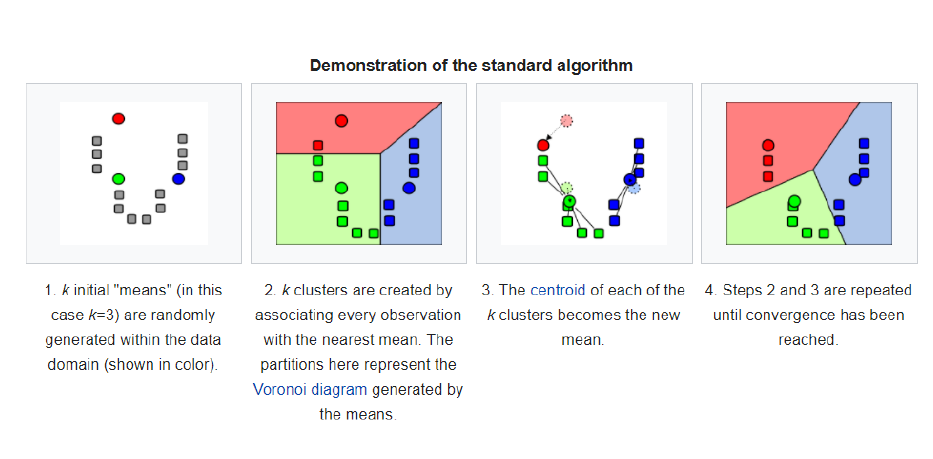
\includegraphics{./pic/chapter-3-0_pic_5.png}
\caption{chapter-3-0\_pic\_5.png}
\end{figure}

    \hypertarget{how-the-k-means-algorithm-works}{%
\paragraph{How the K-means algorithm
works}\label{how-the-k-means-algorithm-works}}

To process the learning data, the K-means algorithm in data mining
starts with a first group of randomly selected centroids, which are used
as the beginning points for every cluster, and then performs iterative
(repetitive) calculations to optimize the positions of the centroids. It
halts creating and optimizing clusters when either:

\begin{itemize}
\tightlist
\item
  The centroids have stabilized --- there is no change in their values
  because the clustering has been successful.
\item
  The defined number of iterations has been achieved.
\end{itemize}

\hypertarget{a-distance-measure}{%
\paragraph{A Distance Measure}\label{a-distance-measure}}

For clustering we need a distance measure. The simplest distance measure
is the Euclidean Distance measure:

\[
Distance = \sqrt{(x_B-x_B)^2 + (y_B - y_A)^2}
\]

\hypertarget{k-means-algorithm-example-problem}{%
\paragraph{K-means algorithm example
problem}\label{k-means-algorithm-example-problem}}

Let's see the steps on how the K-means machine learning algorithm works
using the Python programming language. We'll use the Scikit-learn
library and some random data to illustrate a K-means clustering simple
explanation.

    \begin{tcolorbox}[breakable, size=fbox, boxrule=1pt, pad at break*=1mm,colback=cellbackground, colframe=cellborder]
\prompt{In}{incolor}{1}{\boxspacing}
\begin{Verbatim}[commandchars=\\\{\}]
\PY{k+kn}{import} \PY{n+nn}{pandas} \PY{k}{as} \PY{n+nn}{pd}
\PY{k+kn}{import} \PY{n+nn}{numpy} \PY{k}{as} \PY{n+nn}{np}
\PY{k+kn}{import} \PY{n+nn}{matplotlib}\PY{n+nn}{.}\PY{n+nn}{pyplot} \PY{k}{as} \PY{n+nn}{plt}
\PY{k+kn}{from} \PY{n+nn}{sklearn}\PY{n+nn}{.}\PY{n+nn}{cluster} \PY{k+kn}{import} \PY{n}{KMeans}
\PY{o}{\PYZpc{}}\PY{k}{matplotlib} inline
\end{Verbatim}
\end{tcolorbox}

    Here is the code for generating some random data in a two-dimensional
space:

    \begin{tcolorbox}[breakable, size=fbox, boxrule=1pt, pad at break*=1mm,colback=cellbackground, colframe=cellborder]
\prompt{In}{incolor}{2}{\boxspacing}
\begin{Verbatim}[commandchars=\\\{\}]
\PY{n}{X}  \PY{o}{=}    \PY{o}{\PYZhy{}}\PY{l+m+mi}{2} \PY{o}{*} \PY{n}{np}\PY{o}{.}\PY{n}{random}\PY{o}{.}\PY{n}{rand}\PY{p}{(}\PY{l+m+mi}{100}\PY{p}{,}\PY{l+m+mi}{2}\PY{p}{)}
\PY{n}{X1} \PY{o}{=} \PY{l+m+mi}{1} \PY{o}{+} \PY{l+m+mi}{2} \PY{o}{*} \PY{n}{np}\PY{o}{.}\PY{n}{random}\PY{o}{.}\PY{n}{rand}\PY{p}{(}\PY{l+m+mi}{50}\PY{p}{,}\PY{l+m+mi}{2}\PY{p}{)}
\PY{n}{X}\PY{p}{[}\PY{l+m+mi}{50}\PY{p}{:}\PY{l+m+mi}{100}\PY{p}{,} \PY{p}{:}\PY{p}{]} \PY{o}{=} \PY{n}{X1}
\PY{n}{plt}\PY{o}{.}\PY{n}{scatter}\PY{p}{(}\PY{n}{X}\PY{p}{[} \PY{p}{:} \PY{p}{,} \PY{l+m+mi}{0}\PY{p}{]}\PY{p}{,} \PY{n}{X}\PY{p}{[} \PY{p}{:}\PY{p}{,} \PY{l+m+mi}{1}\PY{p}{]}\PY{p}{,} \PY{n}{s} \PY{o}{=} \PY{l+m+mi}{10}\PY{p}{,} \PY{n}{c} \PY{o}{=} \PY{l+s+s1}{\PYZsq{}}\PY{l+s+s1}{b}\PY{l+s+s1}{\PYZsq{}}\PY{p}{)}
\PY{n}{plt}\PY{o}{.}\PY{n}{grid}\PY{p}{(}\PY{p}{)}
\PY{n}{plt}\PY{o}{.}\PY{n}{show}\PY{p}{(}\PY{p}{)}
\end{Verbatim}
\end{tcolorbox}

    \begin{center}
    \adjustimage{max size={0.9\linewidth}{0.9\paperheight}}{output_9_0.png}
    \end{center}
    { \hspace*{\fill} \\}
    
    This give us two sets approximately centered about (-1,-1) and (2, 2).
We'll use some of the available functions in the Scikit-learn library to
process the randomly generated data.

    \begin{tcolorbox}[breakable, size=fbox, boxrule=1pt, pad at break*=1mm,colback=cellbackground, colframe=cellborder]
\prompt{In}{incolor}{3}{\boxspacing}
\begin{Verbatim}[commandchars=\\\{\}]
\PY{k+kn}{from} \PY{n+nn}{sklearn}\PY{n+nn}{.}\PY{n+nn}{cluster} \PY{k+kn}{import} \PY{n}{KMeans}
\PY{n}{Kmean} \PY{o}{=} \PY{n}{KMeans}\PY{p}{(}\PY{n}{n\PYZus{}clusters}\PY{o}{=}\PY{l+m+mi}{2}\PY{p}{)}
\PY{n}{Kmean}\PY{o}{.}\PY{n}{fit}\PY{p}{(}\PY{n}{X}\PY{p}{)}
\end{Verbatim}
\end{tcolorbox}

            \begin{tcolorbox}[breakable, size=fbox, boxrule=.5pt, pad at break*=1mm, opacityfill=0]
\prompt{Out}{outcolor}{3}{\boxspacing}
\begin{Verbatim}[commandchars=\\\{\}]
KMeans(n\_clusters=2)
\end{Verbatim}
\end{tcolorbox}
        
    In this case, we arbitrarily gave k (n\_clusters) an arbitrary value of
two. Here is the output of the K-means parameters we get if we run the
code:

    \begin{tcolorbox}[breakable, size=fbox, boxrule=1pt, pad at break*=1mm,colback=cellbackground, colframe=cellborder]
\prompt{In}{incolor}{29}{\boxspacing}
\begin{Verbatim}[commandchars=\\\{\}]
\PY{c+c1}{\PYZsh{}KMeans(algorithm=\PYZsq{}auto\PYZsq{}, copy\PYZus{}x=True, init=\PYZsq{}k\PYZhy{}means++\PYZsq{}, max\PYZus{}iter=300,}
\PY{c+c1}{\PYZsh{} n\PYZus{}clusters=2, n\PYZus{}init=10, n\PYZus{}jobs=1, precompute\PYZus{}distances=\PYZsq{}auto\PYZsq{},}
\PY{c+c1}{\PYZsh{} random\PYZus{}state=None, tol=0.0001, verbose=0)}
\end{Verbatim}
\end{tcolorbox}

    \begin{tcolorbox}[breakable, size=fbox, boxrule=1pt, pad at break*=1mm,colback=cellbackground, colframe=cellborder]
\prompt{In}{incolor}{30}{\boxspacing}
\begin{Verbatim}[commandchars=\\\{\}]
\PY{n}{KMeans}\PY{p}{(}\PY{n}{max\PYZus{}iter}\PY{o}{=}\PY{l+m+mi}{300}\PY{p}{,} \PY{n}{n\PYZus{}clusters}\PY{o}{=}\PY{l+m+mi}{2}\PY{p}{,} \PY{n}{tol}\PY{o}{=}\PY{l+m+mf}{0.0001}\PY{p}{)}
\end{Verbatim}
\end{tcolorbox}

            \begin{tcolorbox}[breakable, size=fbox, boxrule=.5pt, pad at break*=1mm, opacityfill=0]
\prompt{Out}{outcolor}{30}{\boxspacing}
\begin{Verbatim}[commandchars=\\\{\}]
KMeans(n\_clusters=2)
\end{Verbatim}
\end{tcolorbox}
        
    \begin{tcolorbox}[breakable, size=fbox, boxrule=1pt, pad at break*=1mm,colback=cellbackground, colframe=cellborder]
\prompt{In}{incolor}{31}{\boxspacing}
\begin{Verbatim}[commandchars=\\\{\}]
\PY{n}{Kmean}\PY{o}{.}\PY{n}{cluster\PYZus{}centers\PYZus{}}
\end{Verbatim}
\end{tcolorbox}

            \begin{tcolorbox}[breakable, size=fbox, boxrule=.5pt, pad at break*=1mm, opacityfill=0]
\prompt{Out}{outcolor}{31}{\boxspacing}
\begin{Verbatim}[commandchars=\\\{\}]
array([[ 2.11896647,  2.04141105],
       [-1.02802583, -0.98355376]])
\end{Verbatim}
\end{tcolorbox}
        
    Let's display the cluster centroids

    \begin{tcolorbox}[breakable, size=fbox, boxrule=1pt, pad at break*=1mm,colback=cellbackground, colframe=cellborder]
\prompt{In}{incolor}{32}{\boxspacing}
\begin{Verbatim}[commandchars=\\\{\}]
\PY{n}{plt}\PY{o}{.}\PY{n}{scatter}\PY{p}{(}\PY{n}{X}\PY{p}{[} \PY{p}{:} \PY{p}{,} \PY{l+m+mi}{0}\PY{p}{]}\PY{p}{,} \PY{n}{X}\PY{p}{[} \PY{p}{:} \PY{p}{,} \PY{l+m+mi}{1}\PY{p}{]}\PY{p}{,} \PY{n}{s} \PY{o}{=}\PY{l+m+mi}{10}\PY{p}{,} \PY{n}{c}\PY{o}{=}\PY{l+s+s1}{\PYZsq{}}\PY{l+s+s1}{b}\PY{l+s+s1}{\PYZsq{}}\PY{p}{)}
\PY{n}{plt}\PY{o}{.}\PY{n}{scatter}\PY{p}{(}\PY{o}{\PYZhy{}}\PY{l+m+mf}{0.94665068}\PY{p}{,} \PY{o}{\PYZhy{}}\PY{l+m+mf}{0.97138368}\PY{p}{,} \PY{n}{s}\PY{o}{=}\PY{l+m+mi}{100}\PY{p}{,} \PY{n}{c}\PY{o}{=}\PY{l+s+s1}{\PYZsq{}}\PY{l+s+s1}{g}\PY{l+s+s1}{\PYZsq{}}\PY{p}{,} \PY{n}{marker}\PY{o}{=}\PY{l+s+s1}{\PYZsq{}}\PY{l+s+s1}{s}\PY{l+s+s1}{\PYZsq{}}\PY{p}{)}
\PY{n}{plt}\PY{o}{.}\PY{n}{scatter}\PY{p}{(} \PY{l+m+mf}{2.01559419}\PY{p}{,}  \PY{l+m+mf}{2.02597093}\PY{p}{,} \PY{n}{s}\PY{o}{=}\PY{l+m+mi}{100}\PY{p}{,} \PY{n}{c}\PY{o}{=}\PY{l+s+s1}{\PYZsq{}}\PY{l+s+s1}{r}\PY{l+s+s1}{\PYZsq{}}\PY{p}{,} \PY{n}{marker}\PY{o}{=}\PY{l+s+s1}{\PYZsq{}}\PY{l+s+s1}{s}\PY{l+s+s1}{\PYZsq{}}\PY{p}{)}
\PY{n}{plt}\PY{o}{.}\PY{n}{grid}\PY{p}{(}\PY{p}{)}
\PY{n}{plt}\PY{o}{.}\PY{n}{show}\PY{p}{(}\PY{p}{)}
\end{Verbatim}
\end{tcolorbox}

    \begin{center}
    \adjustimage{max size={0.9\linewidth}{0.9\paperheight}}{output_17_0.png}
    \end{center}
    { \hspace*{\fill} \\}
    
    Here is the code for getting the labels property of the K-means
clustering example dataset; that is, how the data points are categorized
into the two clusters.

    \begin{tcolorbox}[breakable, size=fbox, boxrule=1pt, pad at break*=1mm,colback=cellbackground, colframe=cellborder]
\prompt{In}{incolor}{33}{\boxspacing}
\begin{Verbatim}[commandchars=\\\{\}]
\PY{n}{Kmean}\PY{o}{.}\PY{n}{labels\PYZus{}}
\end{Verbatim}
\end{tcolorbox}

            \begin{tcolorbox}[breakable, size=fbox, boxrule=.5pt, pad at break*=1mm, opacityfill=0]
\prompt{Out}{outcolor}{33}{\boxspacing}
\begin{Verbatim}[commandchars=\\\{\}]
array([1, 1, 1, 1, 1, 1, 1, 1, 1, 1, 1, 1, 1, 1, 1, 1, 1, 1, 1, 1, 1, 1,
       1, 1, 1, 1, 1, 1, 1, 1, 1, 1, 1, 1, 1, 1, 1, 1, 1, 1, 1, 1, 1, 1,
       1, 1, 1, 1, 1, 1, 0, 0, 0, 0, 0, 0, 0, 0, 0, 0, 0, 0, 0, 0, 0, 0,
       0, 0, 0, 0, 0, 0, 0, 0, 0, 0, 0, 0, 0, 0, 0, 0, 0, 0, 0, 0, 0, 0,
       0, 0, 0, 0, 0, 0, 0, 0, 0, 0, 0, 0])
\end{Verbatim}
\end{tcolorbox}
        
    As you can see above, 50 data points belong to the 0 cluster while the
rest belong to the 1 cluster.

    For example, let's use the code below for predicting the cluster of a
data point:

    \begin{tcolorbox}[breakable, size=fbox, boxrule=1pt, pad at break*=1mm,colback=cellbackground, colframe=cellborder]
\prompt{In}{incolor}{34}{\boxspacing}
\begin{Verbatim}[commandchars=\\\{\}]
\PY{n}{sample\PYZus{}test}\PY{o}{=}\PY{n}{np}\PY{o}{.}\PY{n}{array}\PY{p}{(}\PY{p}{[}\PY{l+m+mf}{1.5}\PY{p}{,}\PY{l+m+mf}{1.5}\PY{p}{]}\PY{p}{)}
\PY{n}{second\PYZus{}test}\PY{o}{=}\PY{n}{sample\PYZus{}test}\PY{o}{.}\PY{n}{reshape}\PY{p}{(}\PY{l+m+mi}{1}\PY{p}{,} \PY{o}{\PYZhy{}}\PY{l+m+mi}{1}\PY{p}{)}
\PY{n}{Kmean}\PY{o}{.}\PY{n}{predict}\PY{p}{(}\PY{n}{second\PYZus{}test}\PY{p}{)}
\end{Verbatim}
\end{tcolorbox}

            \begin{tcolorbox}[breakable, size=fbox, boxrule=.5pt, pad at break*=1mm, opacityfill=0]
\prompt{Out}{outcolor}{34}{\boxspacing}
\begin{Verbatim}[commandchars=\\\{\}]
array([0])
\end{Verbatim}
\end{tcolorbox}
        
    \hypertarget{example-2---country-risk}{%
\subsubsection{Example 2 - Country
Risk}\label{example-2---country-risk}}

    \begin{tcolorbox}[breakable, size=fbox, boxrule=1pt, pad at break*=1mm,colback=cellbackground, colframe=cellborder]
\prompt{In}{incolor}{35}{\boxspacing}
\begin{Verbatim}[commandchars=\\\{\}]
\PY{c+c1}{\PYZsh{} loading packages }

\PY{k+kn}{import} \PY{n+nn}{os}

\PY{k+kn}{import} \PY{n+nn}{pandas} \PY{k}{as} \PY{n+nn}{pd}
\PY{k+kn}{import} \PY{n+nn}{numpy} \PY{k}{as} \PY{n+nn}{np}

\PY{c+c1}{\PYZsh{} plotting packages}
\PY{o}{\PYZpc{}}\PY{k}{matplotlib} inline
\PY{k+kn}{from} \PY{n+nn}{mpl\PYZus{}toolkits}\PY{n+nn}{.}\PY{n+nn}{mplot3d} \PY{k+kn}{import} \PY{n}{Axes3D}
\PY{k+kn}{import} \PY{n+nn}{matplotlib}\PY{n+nn}{.}\PY{n+nn}{pyplot} \PY{k}{as} \PY{n+nn}{plt}
\PY{k+kn}{import} \PY{n+nn}{matplotlib}\PY{n+nn}{.}\PY{n+nn}{cm} \PY{k}{as} \PY{n+nn}{cm}
\PY{k+kn}{import} \PY{n+nn}{matplotlib}\PY{n+nn}{.}\PY{n+nn}{colors} \PY{k}{as} \PY{n+nn}{clrs}

\PY{c+c1}{\PYZsh{} Kmeans algorithm from scikit\PYZhy{}learn}
\PY{k+kn}{from} \PY{n+nn}{sklearn}\PY{n+nn}{.}\PY{n+nn}{cluster} \PY{k+kn}{import} \PY{n}{KMeans}
\PY{k+kn}{from} \PY{n+nn}{sklearn}\PY{n+nn}{.}\PY{n+nn}{metrics} \PY{k+kn}{import} \PY{n}{silhouette\PYZus{}samples}\PY{p}{,} \PY{n}{silhouette\PYZus{}score}
\end{Verbatim}
\end{tcolorbox}

    \hypertarget{the-country-risk-dataset-j.-c.-hull-2019-chapter-2}{%
\paragraph{The Country Risk Dataset (J. C. Hull, 2019, Chapter
2)}\label{the-country-risk-dataset-j.-c.-hull-2019-chapter-2}}

Consider the problem of understanding the risk of countries for foreign
investment. Among the features that can be used for this are:

\begin{itemize}
\tightlist
\item
  GDP growth rate (IMF)
\item
  Corruption index (Transparency international)
\item
  Peace index (Institute for Economics and Peace)
\item
  Legal Risk Index (Property Rights Association)
\end{itemize}

Values for each of the features for 122 countries are found in the
\texttt{countryriskdata.csv} (available
\href{http://www-2.rotman.utoronto.ca/~hull}{here})

    \begin{tcolorbox}[breakable, size=fbox, boxrule=1pt, pad at break*=1mm,colback=cellbackground, colframe=cellborder]
\prompt{In}{incolor}{36}{\boxspacing}
\begin{Verbatim}[commandchars=\\\{\}]
\PY{k}{if} \PY{l+s+s1}{\PYZsq{}}\PY{l+s+s1}{google.colab}\PY{l+s+s1}{\PYZsq{}} \PY{o+ow}{in} \PY{n+nb}{str}\PY{p}{(}\PY{n}{get\PYZus{}ipython}\PY{p}{(}\PY{p}{)}\PY{p}{)}\PY{p}{:}
    \PY{k+kn}{from} \PY{n+nn}{google}\PY{n+nn}{.}\PY{n+nn}{colab} \PY{k+kn}{import} \PY{n}{files}
    \PY{n}{uploaded} \PY{o}{=} \PY{n}{files}\PY{o}{.}\PY{n}{upload}\PY{p}{(}\PY{p}{)}
    \PY{n}{path} \PY{o}{=} \PY{l+s+s1}{\PYZsq{}}\PY{l+s+s1}{\PYZsq{}}
\PY{k}{else}\PY{p}{:}
    \PY{n}{path} \PY{o}{=} \PY{l+s+s1}{\PYZsq{}}\PY{l+s+s1}{./data/}\PY{l+s+s1}{\PYZsq{}}
\end{Verbatim}
\end{tcolorbox}

    \begin{tcolorbox}[breakable, size=fbox, boxrule=1pt, pad at break*=1mm,colback=cellbackground, colframe=cellborder]
\prompt{In}{incolor}{37}{\boxspacing}
\begin{Verbatim}[commandchars=\\\{\}]
\PY{c+c1}{\PYZsh{} load raw data}
\PY{n}{raw} \PY{o}{=} \PY{n}{pd}\PY{o}{.}\PY{n}{read\PYZus{}csv}\PY{p}{(}\PY{n}{os}\PY{o}{.}\PY{n}{path}\PY{o}{.}\PY{n}{join}\PY{p}{(}\PY{n}{path}\PY{p}{,} \PY{l+s+s1}{\PYZsq{}}\PY{l+s+s1}{countryriskdata.csv}\PY{l+s+s1}{\PYZsq{}}\PY{p}{)}\PY{p}{)}

\PY{c+c1}{\PYZsh{} check the raw data}
\PY{n+nb}{print}\PY{p}{(}\PY{l+s+s2}{\PYZdq{}}\PY{l+s+s2}{Size of the dataset (row, col): }\PY{l+s+s2}{\PYZdq{}}\PY{p}{,} \PY{n}{raw}\PY{o}{.}\PY{n}{shape}\PY{p}{)}
\PY{n+nb}{print}\PY{p}{(}\PY{l+s+s2}{\PYZdq{}}\PY{l+s+se}{\PYZbs{}n}\PY{l+s+s2}{First 5 rows}\PY{l+s+se}{\PYZbs{}n}\PY{l+s+s2}{\PYZdq{}}\PY{p}{,} \PY{n}{raw}\PY{o}{.}\PY{n}{head}\PY{p}{(}\PY{n}{n}\PY{o}{=}\PY{l+m+mi}{5}\PY{p}{)}\PY{p}{)}
\end{Verbatim}
\end{tcolorbox}

    \begin{Verbatim}[commandchars=\\\{\}]
Size of the dataset (row, col):  (122, 6)

First 5 rows
      Country Abbrev  Corruption  Peace  Legal  GDP Growth
0    Albania     AL          39  1.867  3.822       3.403
1    Algeria     DZ          34  2.213  4.160       4.202
2  Argentina     AR          36  1.957  4.568      -2.298
3    Armenia     AM          33  2.218  4.126       0.208
4  Australia     AU          79  1.465  8.244       2.471
    \end{Verbatim}

    The GDP growth rate (\%) is typically a positive or negative number with
a magnitude less than 10. The corruption index is on a scale from 0
(highly corrupt) to 100 (no corruption). The peace index is on a scale
from 1 (very peaceful) to 5 (not at all peaceful). The legal risk index
runs from 0 to 10 (with high values being favorable).

    \hypertarget{simple-exploratory-analysis}{%
\subsubsection{Simple exploratory
analysis}\label{simple-exploratory-analysis}}

\textbf{Print summary statistics}

Note that all features have quite different variances, and Corruption
and Legal are highly correlated.

    \begin{tcolorbox}[breakable, size=fbox, boxrule=1pt, pad at break*=1mm,colback=cellbackground, colframe=cellborder]
\prompt{In}{incolor}{38}{\boxspacing}
\begin{Verbatim}[commandchars=\\\{\}]
\PY{c+c1}{\PYZsh{} print summary statistics}
\PY{n+nb}{print}\PY{p}{(}\PY{l+s+s2}{\PYZdq{}}\PY{l+s+se}{\PYZbs{}n}\PY{l+s+s2}{Summary statistics}\PY{l+s+se}{\PYZbs{}n}\PY{l+s+s2}{\PYZdq{}}\PY{p}{,} \PY{n}{raw}\PY{o}{.}\PY{n}{describe}\PY{p}{(}\PY{p}{)}\PY{p}{)}
\PY{n+nb}{print}\PY{p}{(}\PY{l+s+s2}{\PYZdq{}}\PY{l+s+se}{\PYZbs{}n}\PY{l+s+s2}{Correlation matrix}\PY{l+s+se}{\PYZbs{}n}\PY{l+s+s2}{\PYZdq{}}\PY{p}{,} \PY{n}{raw}\PY{o}{.}\PY{n}{corr}\PY{p}{(}\PY{p}{)}\PY{p}{)}
\end{Verbatim}
\end{tcolorbox}

    \begin{Verbatim}[commandchars=\\\{\}]

Summary statistics
        Corruption       Peace       Legal  GDP Growth
count  122.000000  122.000000  122.000000  122.000000
mean    46.237705    2.003730    5.598861    2.372566
std     19.126397    0.447826    1.487328    3.241424
min     14.000000    1.192000    2.728000  -18.000000
25\%     31.250000    1.684750    4.571750    1.432250
50\%     40.000000    1.969000    5.274000    2.496000
75\%     58.750000    2.280500    6.476750    4.080000
max     90.000000    3.399000    8.633000    7.958000

Correlation matrix
             Corruption     Peace     Legal  GDP Growth
Corruption    1.000000 -0.700477  0.923589    0.102513
Peace        -0.700477  1.000000 -0.651961   -0.199855
Legal         0.923589 -0.651961  1.000000    0.123440
GDP Growth    0.102513 -0.199855  0.123440    1.000000
    \end{Verbatim}

    \textbf{Plot histogram}

Note that distributions for GDP Growth is quite skewed.

    \begin{tcolorbox}[breakable, size=fbox, boxrule=1pt, pad at break*=1mm,colback=cellbackground, colframe=cellborder]
\prompt{In}{incolor}{39}{\boxspacing}
\begin{Verbatim}[commandchars=\\\{\}]
\PY{c+c1}{\PYZsh{} plot histograms}
\PY{n}{plt}\PY{o}{.}\PY{n}{figure}\PY{p}{(}\PY{l+m+mi}{1}\PY{p}{)}
\PY{n}{raw}\PY{p}{[}\PY{l+s+s1}{\PYZsq{}}\PY{l+s+s1}{Corruption}\PY{l+s+s1}{\PYZsq{}}\PY{p}{]}\PY{o}{.}\PY{n}{plot}\PY{p}{(}\PY{n}{kind} \PY{o}{=} \PY{l+s+s1}{\PYZsq{}}\PY{l+s+s1}{hist}\PY{l+s+s1}{\PYZsq{}}\PY{p}{,} \PY{n}{title} \PY{o}{=} \PY{l+s+s1}{\PYZsq{}}\PY{l+s+s1}{Corruption}\PY{l+s+s1}{\PYZsq{}}\PY{p}{,} \PY{n}{alpha} \PY{o}{=} \PY{l+m+mf}{0.5}\PY{p}{)}

\PY{n}{plt}\PY{o}{.}\PY{n}{figure}\PY{p}{(}\PY{l+m+mi}{2}\PY{p}{)}
\PY{n}{raw}\PY{p}{[}\PY{l+s+s1}{\PYZsq{}}\PY{l+s+s1}{Peace}\PY{l+s+s1}{\PYZsq{}}\PY{p}{]}\PY{o}{.}\PY{n}{plot}\PY{p}{(}\PY{n}{kind} \PY{o}{=} \PY{l+s+s1}{\PYZsq{}}\PY{l+s+s1}{hist}\PY{l+s+s1}{\PYZsq{}}\PY{p}{,} \PY{n}{title} \PY{o}{=} \PY{l+s+s1}{\PYZsq{}}\PY{l+s+s1}{Peace}\PY{l+s+s1}{\PYZsq{}}\PY{p}{,} \PY{n}{alpha} \PY{o}{=} \PY{l+m+mf}{0.5}\PY{p}{)}

\PY{n}{plt}\PY{o}{.}\PY{n}{figure}\PY{p}{(}\PY{l+m+mi}{3}\PY{p}{)}
\PY{n}{raw}\PY{p}{[}\PY{l+s+s1}{\PYZsq{}}\PY{l+s+s1}{Legal}\PY{l+s+s1}{\PYZsq{}}\PY{p}{]}\PY{o}{.}\PY{n}{plot}\PY{p}{(}\PY{n}{kind} \PY{o}{=} \PY{l+s+s1}{\PYZsq{}}\PY{l+s+s1}{hist}\PY{l+s+s1}{\PYZsq{}}\PY{p}{,} \PY{n}{title} \PY{o}{=} \PY{l+s+s1}{\PYZsq{}}\PY{l+s+s1}{Legal}\PY{l+s+s1}{\PYZsq{}}\PY{p}{,} \PY{n}{alpha} \PY{o}{=} \PY{l+m+mf}{0.5}\PY{p}{)}

\PY{n}{plt}\PY{o}{.}\PY{n}{figure}\PY{p}{(}\PY{l+m+mi}{4}\PY{p}{)}
\PY{n}{raw}\PY{p}{[}\PY{l+s+s1}{\PYZsq{}}\PY{l+s+s1}{GDP Growth}\PY{l+s+s1}{\PYZsq{}}\PY{p}{]}\PY{o}{.}\PY{n}{plot}\PY{p}{(}\PY{n}{kind} \PY{o}{=} \PY{l+s+s1}{\PYZsq{}}\PY{l+s+s1}{hist}\PY{l+s+s1}{\PYZsq{}}\PY{p}{,} \PY{n}{title} \PY{o}{=} \PY{l+s+s1}{\PYZsq{}}\PY{l+s+s1}{GDP Growth}\PY{l+s+s1}{\PYZsq{}}\PY{p}{,} \PY{n}{alpha} \PY{o}{=} \PY{l+m+mf}{0.5}\PY{p}{)}

\PY{n}{plt}\PY{o}{.}\PY{n}{show}\PY{p}{(}\PY{p}{)}
\end{Verbatim}
\end{tcolorbox}

    \begin{center}
    \adjustimage{max size={0.9\linewidth}{0.9\paperheight}}{output_32_0.png}
    \end{center}
    { \hspace*{\fill} \\}
    
    \begin{center}
    \adjustimage{max size={0.9\linewidth}{0.9\paperheight}}{output_32_1.png}
    \end{center}
    { \hspace*{\fill} \\}
    
    \begin{center}
    \adjustimage{max size={0.9\linewidth}{0.9\paperheight}}{output_32_2.png}
    \end{center}
    { \hspace*{\fill} \\}
    
    \begin{center}
    \adjustimage{max size={0.9\linewidth}{0.9\paperheight}}{output_32_3.png}
    \end{center}
    { \hspace*{\fill} \\}
    
    \hypertarget{k-means-cluster}{%
\subsubsection{K means cluster}\label{k-means-cluster}}

\textbf{Pick features \& normalization}

Since Corruption and Legal are highly correlated, we drop the Corruption
variable, i.e., we pick three features for this analysis, Peace, Legal
and GDP Grwoth. Let's normalize all the features, effectively making
them equally weighted.

Ref.
\href{https://stats.stackexchange.com/questions/21222/are-mean-normalization-and-feature-scaling-needed-for-k-means-clustering}{Feature
normalization.}

    \begin{tcolorbox}[breakable, size=fbox, boxrule=1pt, pad at break*=1mm,colback=cellbackground, colframe=cellborder]
\prompt{In}{incolor}{40}{\boxspacing}
\begin{Verbatim}[commandchars=\\\{\}]
\PY{n}{X} \PY{o}{=} \PY{n}{raw}\PY{p}{[}\PY{p}{[}\PY{l+s+s1}{\PYZsq{}}\PY{l+s+s1}{Peace}\PY{l+s+s1}{\PYZsq{}}\PY{p}{,} \PY{l+s+s1}{\PYZsq{}}\PY{l+s+s1}{Legal}\PY{l+s+s1}{\PYZsq{}}\PY{p}{,} \PY{l+s+s1}{\PYZsq{}}\PY{l+s+s1}{GDP Growth}\PY{l+s+s1}{\PYZsq{}}\PY{p}{]}\PY{p}{]}
\PY{n}{X} \PY{o}{=} \PY{p}{(}\PY{n}{X} \PY{o}{\PYZhy{}} \PY{n}{X}\PY{o}{.}\PY{n}{mean}\PY{p}{(}\PY{p}{)}\PY{p}{)} \PY{o}{/} \PY{n}{X}\PY{o}{.}\PY{n}{std}\PY{p}{(}\PY{p}{)}
\PY{n+nb}{print}\PY{p}{(}\PY{n}{X}\PY{o}{.}\PY{n}{head}\PY{p}{(}\PY{l+m+mi}{5}\PY{p}{)}\PY{p}{)}
\end{Verbatim}
\end{tcolorbox}

    \begin{Verbatim}[commandchars=\\\{\}]
      Peace     Legal  GDP Growth
0 -0.305319 -1.194666    0.317896
1  0.467304 -0.967413    0.564392
2 -0.104348 -0.693096   -1.440899
3  0.478469 -0.990273   -0.667782
4 -1.202990  1.778450    0.030368
    \end{Verbatim}

    \hypertarget{perform-elbow-method}{%
\subsubsection{Perform elbow method}\label{perform-elbow-method}}

In cluster analysis, the elbow method is a heuristic used in determining
the number of clusters in a data set. The method consists of plotting
the explained variation as a function of the number of clusters, and
picking the elbow of the curve as the number of clusters to use. The
same method can be used to choose the number of parameters in other
data-driven models, such as the number of principal components to
describe a data set.

For example in the following picture k=4 is suggested

In our case, the marginal gain of adding one cluster dropped quite a bit
from k=3 to k=4. We will choose k=3 (not a clear cut though).

Ref.
\href{https://en.wikipedia.org/wiki/Determining_the_number_of_clusters_in_a_data_set}{Determining
the number of clusters in a dataset.}

    \begin{tcolorbox}[breakable, size=fbox, boxrule=1pt, pad at break*=1mm,colback=cellbackground, colframe=cellborder]
\prompt{In}{incolor}{41}{\boxspacing}
\begin{Verbatim}[commandchars=\\\{\}]
\PY{c+c1}{\PYZsh{} https://stackoverflow.com/questions/41540751/sklearn\PYZhy{}kmeans\PYZhy{}equivalent\PYZhy{}of\PYZhy{}elbow\PYZhy{}method}

\PY{n}{Ks} \PY{o}{=} \PY{n+nb}{range}\PY{p}{(}\PY{l+m+mi}{1}\PY{p}{,} \PY{l+m+mi}{10}\PY{p}{)}
\PY{n}{inertia} \PY{o}{=} \PY{p}{[}\PY{n}{KMeans}\PY{p}{(}\PY{n}{i}\PY{p}{)}\PY{o}{.}\PY{n}{fit}\PY{p}{(}\PY{n}{X}\PY{p}{)}\PY{o}{.}\PY{n}{inertia\PYZus{}} \PY{k}{for} \PY{n}{i} \PY{o+ow}{in} \PY{n}{Ks}\PY{p}{]}

\PY{n}{fig} \PY{o}{=} \PY{n}{plt}\PY{o}{.}\PY{n}{figure}\PY{p}{(}\PY{p}{)}
\PY{n}{plt}\PY{o}{.}\PY{n}{plot}\PY{p}{(}\PY{n}{Ks}\PY{p}{,} \PY{n}{inertia}\PY{p}{,} \PY{l+s+s1}{\PYZsq{}}\PY{l+s+s1}{\PYZhy{}bo}\PY{l+s+s1}{\PYZsq{}}\PY{p}{)}
\PY{n}{plt}\PY{o}{.}\PY{n}{xlabel}\PY{p}{(}\PY{l+s+s1}{\PYZsq{}}\PY{l+s+s1}{Number of clusters}\PY{l+s+s1}{\PYZsq{}}\PY{p}{)}
\PY{n}{plt}\PY{o}{.}\PY{n}{ylabel}\PY{p}{(}\PY{l+s+s1}{\PYZsq{}}\PY{l+s+s1}{Inertia (within\PYZhy{}cluster sum of squares)}\PY{l+s+s1}{\PYZsq{}}\PY{p}{)}
\PY{n}{plt}\PY{o}{.}\PY{n}{show}\PY{p}{(}\PY{p}{)}
\end{Verbatim}
\end{tcolorbox}

    \begin{center}
    \adjustimage{max size={0.9\linewidth}{0.9\paperheight}}{output_36_0.png}
    \end{center}
    { \hspace*{\fill} \\}
    
    \textbf{\emph{k}-means with k=3}

    \begin{tcolorbox}[breakable, size=fbox, boxrule=1pt, pad at break*=1mm,colback=cellbackground, colframe=cellborder]
\prompt{In}{incolor}{42}{\boxspacing}
\begin{Verbatim}[commandchars=\\\{\}]
\PY{n}{k} \PY{o}{=} \PY{l+m+mi}{3}
\PY{n}{kmeans} \PY{o}{=} \PY{n}{KMeans}\PY{p}{(}\PY{n}{n\PYZus{}clusters}\PY{o}{=}\PY{n}{k}\PY{p}{,} \PY{n}{random\PYZus{}state}\PY{o}{=}\PY{l+m+mi}{0}\PY{p}{)}
\PY{n}{kmeans}\PY{o}{.}\PY{n}{fit}\PY{p}{(}\PY{n}{X}\PY{p}{)}

\PY{c+c1}{\PYZsh{} print inertia \PYZam{} cluster center}
\PY{n+nb}{print}\PY{p}{(}\PY{l+s+s2}{\PYZdq{}}\PY{l+s+s2}{inertia for k=3 is}\PY{l+s+s2}{\PYZdq{}}\PY{p}{,} \PY{n}{kmeans}\PY{o}{.}\PY{n}{inertia\PYZus{}}\PY{p}{)}
\PY{n+nb}{print}\PY{p}{(}\PY{l+s+s2}{\PYZdq{}}\PY{l+s+s2}{cluster centers: }\PY{l+s+s2}{\PYZdq{}}\PY{p}{,} \PY{n}{kmeans}\PY{o}{.}\PY{n}{cluster\PYZus{}centers\PYZus{}}\PY{p}{)}

\PY{c+c1}{\PYZsh{} take a quick look at the result}
\PY{n}{y} \PY{o}{=} \PY{n}{kmeans}\PY{o}{.}\PY{n}{labels\PYZus{}}
\PY{n+nb}{print}\PY{p}{(}\PY{l+s+s2}{\PYZdq{}}\PY{l+s+s2}{cluster labels: }\PY{l+s+s2}{\PYZdq{}}\PY{p}{,} \PY{n}{y}\PY{p}{)}
\end{Verbatim}
\end{tcolorbox}

    \begin{Verbatim}[commandchars=\\\{\}]
inertia for k=3 is 157.551489241025
cluster centers:  [[-0.92810589  1.16641329 -0.01445833]
 [ 1.21562552 -1.01677118 -1.61496953]
 [ 0.25320926 -0.45186802  0.43127408]]
cluster labels:  [2 2 1 1 0 0 1 2 2 0 2 2 2 0 1 2 1 2 0 1 0 2 2 0 2 2 0 1 0 2 1
2 2 0 2 0 0
 2 2 0 2 2 2 2 0 0 2 2 2 0 2 0 2 0 2 2 2 0 2 2 1 1 0 2 2 0 2 2 0 2 2 2 2 2
 2 0 0 2 1 0 2 2 2 2 2 2 0 0 0 2 1 2 2 2 2 2 0 0 0 0 0 2 0 0 0 2 2 2 1 2 2
 2 1 0 0 0 0 1 2 1 2 1]
    \end{Verbatim}

    \textbf{Visualize the result (3D plot)}

    \begin{tcolorbox}[breakable, size=fbox, boxrule=1pt, pad at break*=1mm,colback=cellbackground, colframe=cellborder]
\prompt{In}{incolor}{43}{\boxspacing}
\begin{Verbatim}[commandchars=\\\{\}]
\PY{c+c1}{\PYZsh{} set up the color}
\PY{n}{norm} \PY{o}{=} \PY{n}{clrs}\PY{o}{.}\PY{n}{Normalize}\PY{p}{(}\PY{n}{vmin}\PY{o}{=}\PY{l+m+mf}{0.}\PY{p}{,}\PY{n}{vmax}\PY{o}{=}\PY{n}{y}\PY{o}{.}\PY{n}{max}\PY{p}{(}\PY{p}{)}\PY{p}{)}
\PY{n}{cmap} \PY{o}{=} \PY{n}{cm}\PY{o}{.}\PY{n}{viridis}

\PY{n}{fig} \PY{o}{=} \PY{n}{plt}\PY{o}{.}\PY{n}{figure}\PY{p}{(}\PY{n}{figsize}\PY{o}{=}\PY{p}{(}\PY{l+m+mi}{10}\PY{p}{,} \PY{l+m+mi}{8}\PY{p}{)}\PY{p}{)}
\PY{n}{ax} \PY{o}{=} \PY{n}{fig}\PY{o}{.}\PY{n}{add\PYZus{}subplot}\PY{p}{(}\PY{l+m+mi}{111}\PY{p}{,} \PY{n}{projection}\PY{o}{=}\PY{l+s+s1}{\PYZsq{}}\PY{l+s+s1}{3d}\PY{l+s+s1}{\PYZsq{}}\PY{p}{)}

\PY{n}{ax}\PY{o}{.}\PY{n}{scatter}\PY{p}{(}\PY{n}{X}\PY{o}{.}\PY{n}{iloc}\PY{p}{[}\PY{p}{:}\PY{p}{,}\PY{l+m+mi}{0}\PY{p}{]}\PY{p}{,} \PY{n}{X}\PY{o}{.}\PY{n}{iloc}\PY{p}{[}\PY{p}{:}\PY{p}{,}\PY{l+m+mi}{1}\PY{p}{]}\PY{p}{,} \PY{n}{X}\PY{o}{.}\PY{n}{iloc}\PY{p}{[}\PY{p}{:}\PY{p}{,}\PY{l+m+mi}{2}\PY{p}{]}\PY{p}{,} \PY{n}{c}\PY{o}{=}\PY{n}{cmap}\PY{p}{(}\PY{n}{norm}\PY{p}{(}\PY{n}{y}\PY{p}{)}\PY{p}{)}\PY{p}{,} \PY{n}{marker}\PY{o}{=}\PY{l+s+s1}{\PYZsq{}}\PY{l+s+s1}{o}\PY{l+s+s1}{\PYZsq{}}\PY{p}{)}

\PY{n}{centers} \PY{o}{=} \PY{n}{kmeans}\PY{o}{.}\PY{n}{cluster\PYZus{}centers\PYZus{}}
\PY{n}{ax}\PY{o}{.}\PY{n}{scatter}\PY{p}{(}\PY{n}{centers}\PY{p}{[}\PY{p}{:}\PY{p}{,} \PY{l+m+mi}{0}\PY{p}{]}\PY{p}{,} \PY{n}{centers}\PY{p}{[}\PY{p}{:}\PY{p}{,} \PY{l+m+mi}{1}\PY{p}{]}\PY{p}{,} \PY{n}{c}\PY{o}{=}\PY{l+s+s1}{\PYZsq{}}\PY{l+s+s1}{red}\PY{l+s+s1}{\PYZsq{}}\PY{p}{,} \PY{n}{s}\PY{o}{=}\PY{l+m+mi}{100}\PY{p}{,} \PY{n}{alpha}\PY{o}{=}\PY{l+m+mf}{0.5}\PY{p}{,} \PY{n}{marker}\PY{o}{=}\PY{l+s+s1}{\PYZsq{}}\PY{l+s+s1}{o}\PY{l+s+s1}{\PYZsq{}}\PY{p}{)}

\PY{n}{ax}\PY{o}{.}\PY{n}{set\PYZus{}xlabel}\PY{p}{(}\PY{l+s+s1}{\PYZsq{}}\PY{l+s+s1}{Peace}\PY{l+s+s1}{\PYZsq{}}\PY{p}{)}
\PY{n}{ax}\PY{o}{.}\PY{n}{set\PYZus{}ylabel}\PY{p}{(}\PY{l+s+s1}{\PYZsq{}}\PY{l+s+s1}{Legal}\PY{l+s+s1}{\PYZsq{}}\PY{p}{)}
\PY{n}{ax}\PY{o}{.}\PY{n}{set\PYZus{}zlabel}\PY{p}{(}\PY{l+s+s1}{\PYZsq{}}\PY{l+s+s1}{GDP Growth}\PY{l+s+s1}{\PYZsq{}}\PY{p}{)}

\PY{n}{plt}\PY{o}{.}\PY{n}{show}\PY{p}{(}\PY{p}{)}
\end{Verbatim}
\end{tcolorbox}

    \begin{center}
    \adjustimage{max size={0.9\linewidth}{0.9\paperheight}}{output_40_0.png}
    \end{center}
    { \hspace*{\fill} \\}
    
    \textbf{Visualize the result (3 2D plots)}

    \begin{tcolorbox}[breakable, size=fbox, boxrule=1pt, pad at break*=1mm,colback=cellbackground, colframe=cellborder]
\prompt{In}{incolor}{44}{\boxspacing}
\begin{Verbatim}[commandchars=\\\{\}]
\PY{o}{\PYZpc{}}\PY{k}{matplotlib} inline
\PY{k+kn}{import} \PY{n+nn}{matplotlib}\PY{n+nn}{.}\PY{n+nn}{pyplot} \PY{k}{as} \PY{n+nn}{plt}

\PY{n}{figs} \PY{o}{=} \PY{p}{[}\PY{p}{(}\PY{l+m+mi}{0}\PY{p}{,} \PY{l+m+mi}{1}\PY{p}{)}\PY{p}{,} \PY{p}{(}\PY{l+m+mi}{0}\PY{p}{,} \PY{l+m+mi}{2}\PY{p}{)}\PY{p}{,} \PY{p}{(}\PY{l+m+mi}{1}\PY{p}{,} \PY{l+m+mi}{2}\PY{p}{)}\PY{p}{]}
\PY{n}{labels} \PY{o}{=} \PY{p}{[}\PY{l+s+s1}{\PYZsq{}}\PY{l+s+s1}{Peace}\PY{l+s+s1}{\PYZsq{}}\PY{p}{,} \PY{l+s+s1}{\PYZsq{}}\PY{l+s+s1}{Legal}\PY{l+s+s1}{\PYZsq{}}\PY{p}{,} \PY{l+s+s1}{\PYZsq{}}\PY{l+s+s1}{GDP Growth}\PY{l+s+s1}{\PYZsq{}}\PY{p}{]}

\PY{k}{for} \PY{n}{i} \PY{o+ow}{in} \PY{n+nb}{range}\PY{p}{(}\PY{l+m+mi}{3}\PY{p}{)}\PY{p}{:}
    \PY{n}{fig} \PY{o}{=} \PY{n}{plt}\PY{o}{.}\PY{n}{figure}\PY{p}{(}\PY{n}{i}\PY{p}{)}
    \PY{n}{plt}\PY{o}{.}\PY{n}{scatter}\PY{p}{(}\PY{n}{X}\PY{o}{.}\PY{n}{iloc}\PY{p}{[}\PY{p}{:}\PY{p}{,}\PY{n}{figs}\PY{p}{[}\PY{n}{i}\PY{p}{]}\PY{p}{[}\PY{l+m+mi}{0}\PY{p}{]}\PY{p}{]}\PY{p}{,} \PY{n}{X}\PY{o}{.}\PY{n}{iloc}\PY{p}{[}\PY{p}{:}\PY{p}{,}\PY{n}{figs}\PY{p}{[}\PY{n}{i}\PY{p}{]}\PY{p}{[}\PY{l+m+mi}{1}\PY{p}{]}\PY{p}{]}\PY{p}{,} \PY{n}{c}\PY{o}{=}\PY{n}{cmap}\PY{p}{(}\PY{n}{norm}\PY{p}{(}\PY{n}{y}\PY{p}{)}\PY{p}{)}\PY{p}{,} \PY{n}{s}\PY{o}{=}\PY{l+m+mi}{50}\PY{p}{)}
    \PY{n}{plt}\PY{o}{.}\PY{n}{scatter}\PY{p}{(}\PY{n}{centers}\PY{p}{[}\PY{p}{:}\PY{p}{,} \PY{n}{figs}\PY{p}{[}\PY{n}{i}\PY{p}{]}\PY{p}{[}\PY{l+m+mi}{0}\PY{p}{]}\PY{p}{]}\PY{p}{,} \PY{n}{centers}\PY{p}{[}\PY{p}{:}\PY{p}{,} \PY{n}{figs}\PY{p}{[}\PY{n}{i}\PY{p}{]}\PY{p}{[}\PY{l+m+mi}{1}\PY{p}{]}\PY{p}{]}\PY{p}{,} \PY{n}{c}\PY{o}{=}\PY{l+s+s1}{\PYZsq{}}\PY{l+s+s1}{black}\PY{l+s+s1}{\PYZsq{}}\PY{p}{,} \PY{n}{s}\PY{o}{=}\PY{l+m+mi}{200}\PY{p}{,} \PY{n}{alpha}\PY{o}{=}\PY{l+m+mf}{0.5}\PY{p}{)}
    \PY{n}{plt}\PY{o}{.}\PY{n}{xlabel}\PY{p}{(}\PY{n}{labels}\PY{p}{[}\PY{n}{figs}\PY{p}{[}\PY{n}{i}\PY{p}{]}\PY{p}{[}\PY{l+m+mi}{0}\PY{p}{]}\PY{p}{]}\PY{p}{)}
    \PY{n}{plt}\PY{o}{.}\PY{n}{ylabel}\PY{p}{(}\PY{n}{labels}\PY{p}{[}\PY{n}{figs}\PY{p}{[}\PY{n}{i}\PY{p}{]}\PY{p}{[}\PY{l+m+mi}{1}\PY{p}{]}\PY{p}{]}\PY{p}{)}

\PY{n}{plt}\PY{o}{.}\PY{n}{show}\PY{p}{(}\PY{p}{)}
\end{Verbatim}
\end{tcolorbox}

    \begin{center}
    \adjustimage{max size={0.9\linewidth}{0.9\paperheight}}{output_42_0.png}
    \end{center}
    { \hspace*{\fill} \\}
    
    \begin{center}
    \adjustimage{max size={0.9\linewidth}{0.9\paperheight}}{output_42_1.png}
    \end{center}
    { \hspace*{\fill} \\}
    
    \begin{center}
    \adjustimage{max size={0.9\linewidth}{0.9\paperheight}}{output_42_2.png}
    \end{center}
    { \hspace*{\fill} \\}
    
    \textbf{Visualize the result (3 2D plots)}

plot country abbreviations instead of dots.

    \begin{tcolorbox}[breakable, size=fbox, boxrule=1pt, pad at break*=1mm,colback=cellbackground, colframe=cellborder]
\prompt{In}{incolor}{45}{\boxspacing}
\begin{Verbatim}[commandchars=\\\{\}]
\PY{o}{\PYZpc{}}\PY{k}{matplotlib} inline
\PY{k+kn}{import} \PY{n+nn}{matplotlib}\PY{n+nn}{.}\PY{n+nn}{pyplot} \PY{k}{as} \PY{n+nn}{plt}

\PY{n}{figs} \PY{o}{=} \PY{p}{[}\PY{p}{(}\PY{l+m+mi}{0}\PY{p}{,} \PY{l+m+mi}{1}\PY{p}{)}\PY{p}{,} \PY{p}{(}\PY{l+m+mi}{0}\PY{p}{,} \PY{l+m+mi}{2}\PY{p}{)}\PY{p}{,} \PY{p}{(}\PY{l+m+mi}{1}\PY{p}{,} \PY{l+m+mi}{2}\PY{p}{)}\PY{p}{]}
\PY{n}{labels} \PY{o}{=} \PY{p}{[}\PY{l+s+s1}{\PYZsq{}}\PY{l+s+s1}{Peace}\PY{l+s+s1}{\PYZsq{}}\PY{p}{,} \PY{l+s+s1}{\PYZsq{}}\PY{l+s+s1}{Legal}\PY{l+s+s1}{\PYZsq{}}\PY{p}{,} \PY{l+s+s1}{\PYZsq{}}\PY{l+s+s1}{GDP Growth}\PY{l+s+s1}{\PYZsq{}}\PY{p}{]}
\PY{n}{colors} \PY{o}{=} \PY{p}{[}\PY{l+s+s1}{\PYZsq{}}\PY{l+s+s1}{blue}\PY{l+s+s1}{\PYZsq{}}\PY{p}{,}\PY{l+s+s1}{\PYZsq{}}\PY{l+s+s1}{green}\PY{l+s+s1}{\PYZsq{}}\PY{p}{,} \PY{l+s+s1}{\PYZsq{}}\PY{l+s+s1}{red}\PY{l+s+s1}{\PYZsq{}}\PY{p}{]}

\PY{k}{for} \PY{n}{i} \PY{o+ow}{in} \PY{n+nb}{range}\PY{p}{(}\PY{l+m+mi}{3}\PY{p}{)}\PY{p}{:}
    \PY{n}{fig} \PY{o}{=} \PY{n}{plt}\PY{o}{.}\PY{n}{figure}\PY{p}{(}\PY{n}{i}\PY{p}{,} \PY{n}{figsize}\PY{o}{=}\PY{p}{(}\PY{l+m+mi}{8}\PY{p}{,} \PY{l+m+mi}{8}\PY{p}{)}\PY{p}{)}
    \PY{n}{x\PYZus{}1} \PY{o}{=} \PY{n}{figs}\PY{p}{[}\PY{n}{i}\PY{p}{]}\PY{p}{[}\PY{l+m+mi}{0}\PY{p}{]}
    \PY{n}{x\PYZus{}2} \PY{o}{=} \PY{n}{figs}\PY{p}{[}\PY{n}{i}\PY{p}{]}\PY{p}{[}\PY{l+m+mi}{1}\PY{p}{]}
    \PY{n}{plt}\PY{o}{.}\PY{n}{scatter}\PY{p}{(}\PY{n}{X}\PY{o}{.}\PY{n}{iloc}\PY{p}{[}\PY{p}{:}\PY{p}{,} \PY{n}{x\PYZus{}1}\PY{p}{]}\PY{p}{,} \PY{n}{X}\PY{o}{.}\PY{n}{iloc}\PY{p}{[}\PY{p}{:}\PY{p}{,} \PY{n}{x\PYZus{}2}\PY{p}{]}\PY{p}{,} \PY{n}{c}\PY{o}{=}\PY{n}{y}\PY{p}{,} \PY{n}{s}\PY{o}{=}\PY{l+m+mi}{0}\PY{p}{,} \PY{n}{alpha}\PY{o}{=}\PY{l+m+mi}{0}\PY{p}{)}
    \PY{n}{plt}\PY{o}{.}\PY{n}{scatter}\PY{p}{(}\PY{n}{centers}\PY{p}{[}\PY{p}{:}\PY{p}{,} \PY{n}{x\PYZus{}1}\PY{p}{]}\PY{p}{,} \PY{n}{centers}\PY{p}{[}\PY{p}{:}\PY{p}{,} \PY{n}{x\PYZus{}2}\PY{p}{]}\PY{p}{,} \PY{n}{c}\PY{o}{=}\PY{l+s+s1}{\PYZsq{}}\PY{l+s+s1}{black}\PY{l+s+s1}{\PYZsq{}}\PY{p}{,} \PY{n}{s}\PY{o}{=}\PY{l+m+mi}{200}\PY{p}{,} \PY{n}{alpha}\PY{o}{=}\PY{l+m+mf}{0.5}\PY{p}{)}
    \PY{k}{for} \PY{n}{j} \PY{o+ow}{in} \PY{n+nb}{range}\PY{p}{(}\PY{n}{X}\PY{o}{.}\PY{n}{shape}\PY{p}{[}\PY{l+m+mi}{0}\PY{p}{]}\PY{p}{)}\PY{p}{:}
        \PY{n}{plt}\PY{o}{.}\PY{n}{text}\PY{p}{(}\PY{n}{X}\PY{o}{.}\PY{n}{iloc}\PY{p}{[}\PY{n}{j}\PY{p}{,} \PY{n}{x\PYZus{}1}\PY{p}{]}\PY{p}{,} \PY{n}{X}\PY{o}{.}\PY{n}{iloc}\PY{p}{[}\PY{n}{j}\PY{p}{,} \PY{n}{x\PYZus{}2}\PY{p}{]}\PY{p}{,} \PY{n}{raw}\PY{p}{[}\PY{l+s+s1}{\PYZsq{}}\PY{l+s+s1}{Abbrev}\PY{l+s+s1}{\PYZsq{}}\PY{p}{]}\PY{o}{.}\PY{n}{iloc}\PY{p}{[}\PY{n}{j}\PY{p}{]}\PY{p}{,} 
                 \PY{n}{color}\PY{o}{=}\PY{n}{colors}\PY{p}{[}\PY{n}{y}\PY{p}{[}\PY{n}{j}\PY{p}{]}\PY{p}{]}\PY{p}{,} \PY{n}{weight}\PY{o}{=}\PY{l+s+s1}{\PYZsq{}}\PY{l+s+s1}{semibold}\PY{l+s+s1}{\PYZsq{}}\PY{p}{,} \PY{n}{horizontalalignment} \PY{o}{=} \PY{l+s+s1}{\PYZsq{}}\PY{l+s+s1}{center}\PY{l+s+s1}{\PYZsq{}}\PY{p}{,} \PY{n}{verticalalignment} \PY{o}{=} \PY{l+s+s1}{\PYZsq{}}\PY{l+s+s1}{center}\PY{l+s+s1}{\PYZsq{}}\PY{p}{)}
    \PY{n}{plt}\PY{o}{.}\PY{n}{xlabel}\PY{p}{(}\PY{n}{labels}\PY{p}{[}\PY{n}{x\PYZus{}1}\PY{p}{]}\PY{p}{)}
    \PY{n}{plt}\PY{o}{.}\PY{n}{ylabel}\PY{p}{(}\PY{n}{labels}\PY{p}{[}\PY{n}{x\PYZus{}2}\PY{p}{]}\PY{p}{)}

\PY{n}{plt}\PY{o}{.}\PY{n}{show}\PY{p}{(}\PY{p}{)}
\end{Verbatim}
\end{tcolorbox}

    \begin{center}
    \adjustimage{max size={0.9\linewidth}{0.9\paperheight}}{output_44_0.png}
    \end{center}
    { \hspace*{\fill} \\}
    
    \begin{center}
    \adjustimage{max size={0.9\linewidth}{0.9\paperheight}}{output_44_1.png}
    \end{center}
    { \hspace*{\fill} \\}
    
    \begin{center}
    \adjustimage{max size={0.9\linewidth}{0.9\paperheight}}{output_44_2.png}
    \end{center}
    { \hspace*{\fill} \\}
    
    \hypertarget{list-the-result}{%
\subsubsection{List the result}\label{list-the-result}}

    \begin{tcolorbox}[breakable, size=fbox, boxrule=1pt, pad at break*=1mm,colback=cellbackground, colframe=cellborder]
\prompt{In}{incolor}{ }{\boxspacing}
\begin{Verbatim}[commandchars=\\\{\}]
\PY{n}{result} \PY{o}{=} \PY{n}{pd}\PY{o}{.}\PY{n}{DataFrame}\PY{p}{(}\PY{p}{\PYZob{}}\PY{l+s+s1}{\PYZsq{}}\PY{l+s+s1}{Country}\PY{l+s+s1}{\PYZsq{}}\PY{p}{:}\PY{n}{raw}\PY{p}{[}\PY{l+s+s1}{\PYZsq{}}\PY{l+s+s1}{Country}\PY{l+s+s1}{\PYZsq{}}\PY{p}{]}\PY{p}{,} \PY{l+s+s1}{\PYZsq{}}\PY{l+s+s1}{Abbrev}\PY{l+s+s1}{\PYZsq{}}\PY{p}{:}\PY{n}{raw}\PY{p}{[}\PY{l+s+s1}{\PYZsq{}}\PY{l+s+s1}{Abbrev}\PY{l+s+s1}{\PYZsq{}}\PY{p}{]}\PY{p}{,} \PY{l+s+s1}{\PYZsq{}}\PY{l+s+s1}{Label}\PY{l+s+s1}{\PYZsq{}}\PY{p}{:}\PY{n}{y}\PY{p}{\PYZcb{}}\PY{p}{)}
\PY{k}{with} \PY{n}{pd}\PY{o}{.}\PY{n}{option\PYZus{}context}\PY{p}{(}\PY{l+s+s1}{\PYZsq{}}\PY{l+s+s1}{display.max\PYZus{}rows}\PY{l+s+s1}{\PYZsq{}}\PY{p}{,} \PY{k+kc}{None}\PY{p}{,} \PY{l+s+s1}{\PYZsq{}}\PY{l+s+s1}{display.max\PYZus{}columns}\PY{l+s+s1}{\PYZsq{}}\PY{p}{,} \PY{l+m+mi}{3}\PY{p}{)}\PY{p}{:}
    \PY{n+nb}{print}\PY{p}{(}\PY{n}{result}\PY{o}{.}\PY{n}{sort\PYZus{}values}\PY{p}{(}\PY{l+s+s1}{\PYZsq{}}\PY{l+s+s1}{Label}\PY{l+s+s1}{\PYZsq{}}\PY{p}{)}\PY{p}{)}
\end{Verbatim}
\end{tcolorbox}

    \hypertarget{silhouette-analysis}{%
\subsubsection{Silhouette Analysis}\label{silhouette-analysis}}

    For each observation \(i\) calculate \(a(i)\), the average distance from
other observations in its cluster, and \(b(i)\), the average distance
from observations in the closest other cluster. The silhouette score for
observation \(i\), \(s(i)\), is defined as \begin{equation}
        s(i) = \frac{b(i)-a(i)}{\max[a(i),b(i)]}
\end{equation}

Choose the number of clusters that maximizes the average silhouette
score across all observations

    \begin{tcolorbox}[breakable, size=fbox, boxrule=1pt, pad at break*=1mm,colback=cellbackground, colframe=cellborder]
\prompt{In}{incolor}{ }{\boxspacing}
\begin{Verbatim}[commandchars=\\\{\}]
\PY{c+c1}{\PYZsh{} Silhouette Analysis}
\PY{n}{range\PYZus{}n\PYZus{}clusters} \PY{o}{=} \PY{p}{[}\PY{l+m+mi}{2}\PY{p}{,}\PY{l+m+mi}{3}\PY{p}{,}\PY{l+m+mi}{4}\PY{p}{,}\PY{l+m+mi}{5}\PY{p}{,}\PY{l+m+mi}{6}\PY{p}{,}\PY{l+m+mi}{7}\PY{p}{,}\PY{l+m+mi}{8}\PY{p}{,}\PY{l+m+mi}{9}\PY{p}{,}\PY{l+m+mi}{10}\PY{p}{]}
\PY{n}{silhouette}       \PY{o}{=} \PY{p}{[}\PY{p}{]}
\PY{k}{for} \PY{n}{n\PYZus{}clusters} \PY{o+ow}{in} \PY{n}{range\PYZus{}n\PYZus{}clusters}\PY{p}{:}
    \PY{n}{clusterer}\PY{o}{=}\PY{n}{KMeans}\PY{p}{(}\PY{n}{n\PYZus{}clusters}\PY{o}{=}\PY{n}{n\PYZus{}clusters}\PY{p}{,} \PY{n}{random\PYZus{}state}\PY{o}{=}\PY{l+m+mi}{0}\PY{p}{)}
    \PY{n}{cluster\PYZus{}labels}\PY{o}{=}\PY{n}{clusterer}\PY{o}{.}\PY{n}{fit\PYZus{}predict}\PY{p}{(}\PY{n}{X}\PY{p}{)}
    \PY{n}{silhouette\PYZus{}avg}\PY{o}{=}\PY{n}{silhouette\PYZus{}score}\PY{p}{(}\PY{n}{X}\PY{p}{,}\PY{n}{cluster\PYZus{}labels}\PY{p}{)}
    \PY{n}{silhouette}\PY{o}{.}\PY{n}{append}\PY{p}{(}\PY{n}{silhouette\PYZus{}avg}\PY{p}{)}
    \PY{c+c1}{\PYZsh{}print(\PYZdq{}For n\PYZus{}clusters=\PYZdq{}, n\PYZus{}clusters,}
    \PY{c+c1}{\PYZsh{}      \PYZdq{}The average silhouette\PYZus{}score is :\PYZdq{}, silhouette\PYZus{}avg)}
\end{Verbatim}
\end{tcolorbox}

    \begin{tcolorbox}[breakable, size=fbox, boxrule=1pt, pad at break*=1mm,colback=cellbackground, colframe=cellborder]
\prompt{In}{incolor}{ }{\boxspacing}
\begin{Verbatim}[commandchars=\\\{\}]
\PY{n}{plt}\PY{o}{.}\PY{n}{plot}\PY{p}{(}\PY{n}{range\PYZus{}n\PYZus{}clusters}\PY{p}{,} \PY{n}{silhouette}\PY{p}{)}
\end{Verbatim}
\end{tcolorbox}

    \hypertarget{references}{%
\subsection{References}\label{references}}

    John C. Hull, \textbf{Machine Learning in Business: An Introduction to
the World of Data Science}, Amazon, 2019.

Paul Wilmott, \textbf{Machine Learning: An Applied Mathematics
Introduction}, Panda Ohana Publishing, 2019.


    % Add a bibliography block to the postdoc
    
    
    
\end{document}
